\documentclass[12pt]{article}  
\usepackage{graphicx}
\usepackage{geometry}   %设置页边距的宏包
\usepackage{algpseudocode}
\usepackage{comment}
\usepackage{amsmath, amssymb, amsthm}
\usepackage{enumerate}
\usepackage{enumitem}
\usepackage{framed}
\usepackage{verbatim}
\usepackage{microtype}
\usepackage{kpfonts}
\usepackage{multicol}
\usepackage{amsfonts}
\usepackage{array}
\usepackage{color}
\usepackage{pgf,tikz}
\usepackage{mathtools}
\usetikzlibrary{automata, positioning, arrows}
\usepackage{wrapfig}
\newcommand{\solu}{{\color{blue} Solution:}}
\newcommand{\overbar}[1]{\mkern 1.5mu\overline{\mkern-1.5mu#1\mkern-1.5mu}\mkern 1.5mu}
\newcommand{\Ib}{\mathbf{I}}
\newcommand{\Pb}{\mathbf{P}}
\newcommand{\Qb}{\mathbf{Q}}
\newcommand{\Rb}{\mathbf{R}}
\newcommand{\Nb}{\mathbf{N}}
\newcommand{\Fb}{\mathbf{F}}
\newcommand{\Z}{\mathbf{Z}}
\newcommand{\Lap}{\mathcal{L}}
\newcommand{\Zplus}{\mathbf{Z}^+}
\newcommand{\indep}{\perp \!\!\! \perp}
\DeclareMathOperator*{\argmin}{\arg\min}
\DeclareMathOperator*{\argmax}{\arg\max}
\geometry{left=1.5cm,right=1.5cm,top=1.5cm,bottom=1.5cm}  %设置 上、左、下、右 页边距
\tikzset{
    ->, % makes the edges directed
    >=stealth, % makes the arrow heads bold
    node distance=3cm, % specifies the minimum distance between two nodes. Change if necessary.
    every state/.style={thick, fill=gray!10}, % sets the properties for each ’state’ node
    initial text=$ $, % sets the text that appears on the start arrow
} 
\title{DS4400 HW4}
\author{Xin Guan}
\date{}

\begin{document}
    \maketitle
    \begin{enumerate}
        \item \textbf{SVM}. Consider a supervised learning problem in which the training examples are points in 2-dimensional space. The positive examples (samples in class 1) are $(1, 1)$ and $(-1, -1)$. The negative examples (samples in class 0) are $(1, -1)$ and $(-1, 1)$. Are the positive examples linearly separable from the negative examples in the original space? If so, give the coefficients of $\omega$.
        \begin{enumerate}
            \item For the example above, consider the feature transformation $\phi(x) = [1, x_1, x_2, x_1x_2]$, where $x_1$ and $x_2$ are, respectively, the first and second coordinates of a generic example $x$. Can we find a hyperplance $\omega^T\phi(x)$ in this feature space that can separate the data from positive and negative class. If so, give the coefficients of $\omega$ (You should be able to do this by inspection, without significant computation).
            
            \solu 

            We find that when $x_1, x_2$ have the same sign, they belong to +. If $x_1, x_2$ have different sign, they belong to $-$ Therefore, we can use $x_1x_2$ to decide its category. Then we can pick $\omega = [0,0,0,1]$.

            \item What is the kernel corresponding to the feature map $\phi(\cdot)$ in the last part. In other words provde the kernel function $K(x,z) = \mathbb{R}^2 \times \mathbb{R}^2 \rightarrow \mathbb{R}$
            
            \solu 

            $K(x,z) = [1,x_1, x_2, x_1x_2]^T\cdot[1,z_1,z_2,z_1z_2] = 1 +x_1z_1 + x_2z_2 + x_1x_2z_1z_2 = 1 + xz + \frac{(xz)^2 - ||xz||_2^2}{2}$
            
        \end{enumerate}

        \item \textbf{Neural Network} Consider a neural net for a binary classification which has one hidden layer as shown in the figure below. We use a linear activation function $a(z) = cz$ at hidden units and a sigmoid activation function $a(z) = 1/(1 + e^{-z})$ at the output unit to learn the function for $P(y = 1|x, w)$ where $x = (x_1, x_2)$ and $w = (w_1, w_2, \dots , w_9)$.
        \begin{enumerate}
            \item What is the output $P(y = 1|x, w)$ from the above neural net? Express it in terms of $x_i, $c and weights $w_i$. What is the final classification boundary?
            
            \solu 

            For the first neuron of the hidden level: $A = a_1(w_1 + x_1w_3 + x_2w_5) = c(w_1 + x_1w_3 + x_2w_5)$. For the second neuron of the hidden level: $B = a_1(w_2 + x_1w_4 + x_2w_6) = c(w_2 + x_1w_4 + x_2w_6)$. 
            
            Then the output neuron is $a_2(w_7 + w_8A + w_9B) = \frac{1}{(1 + e^{-(w_7 + w_8(c(w_1 + x_1w_3 + x_2w_5)) + w_9(c(w_2 + x_1w_4 + x_2w_6)))})}$

            The boundary: let $w_7 + w_8A + w_9B = 0$.
            Then we have 
            $$w_7 + w_8(c(w_1 + x_1w_3 + x_2w_5)) + w_9(c(w_2 + x_1w_4 + x_2w_6)) = 0$$
            Or we formulate it as:
            $$(w_8w_3 + w_9w_4)cx_1 + (w_8w_5 +w_9w_6)cx_2 + w_7 + w_1w_8c + w_9w_2c = 0$$
            Therefore,
            $y = \left\{
                \begin{array}{rcl}
                1  & & (w_8w_3 + w_9w_4)cx_1 + (w_8w_5 +w_9w_6)cx_2 + w_7 + w_1w_8c + w_9w_2c > 0 \\
                0 & & (w_8w_3 + w_9w_4)cx_1 + (w_8w_5 +w_9w_6)cx_2 + w_7 + w_1w_8c + w_9w_2c < 0
            \end{array}
            \right.$

            \item Draw a neural net with no hidden layer which is equivalent to the given neural net, and write weights $\tilde{w}$ of this new neural net in terms of $c$ and $w_i$.
            
            \solu 

            \begin{center}
                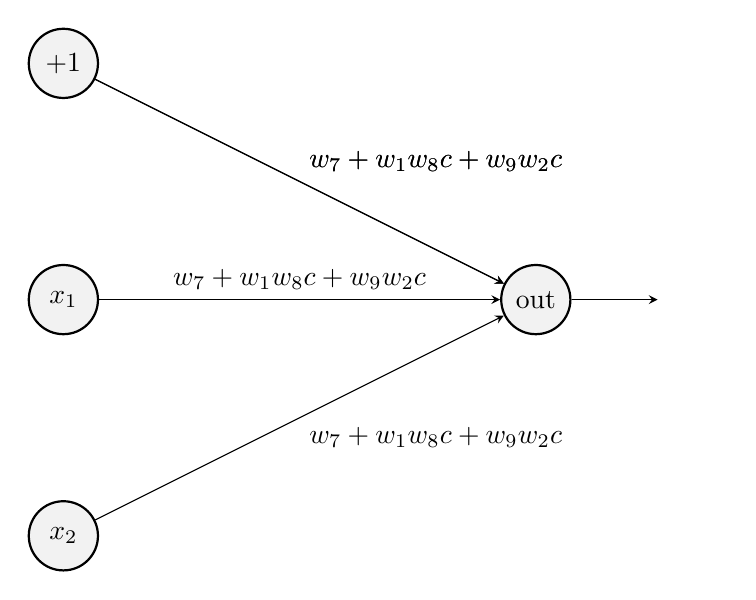
\begin{tikzpicture}
                    \node[state] (1) {+1};
                    \node[state, below of=1] (x1) {$x_1$};
                    \node[state, below of=x1] (x2) {$x_2$};
                    \node[state, right of=x1, node distance=6cm] (o) {out};
                    \node[state, right of=o, draw=none, node distance=2cm, fill=white] (y) {};
                    \draw (1) edge[above right] node{$w_7 + w_1w_8c + w_9w_2c$} (o)
                    (1) edge[above right] node{$w_7 + w_1w_8c + w_9w_2c$} (o)
                    (x1) edge[above] node{$w_7 + w_1w_8c + w_9w_2c$} (o)
                    (x2) edge[below right] node{$w_7 + w_1w_8c + w_9w_2c$} (o)
                    (o) edge[below right] node{$ $} (y);
                \end{tikzpicture}
            \end{center}

            The out node is using a sigmoid function.
            \item Is it true that any multi-layered neural net with linear activation functions at hidden layers can be represented as a neural net without any hidden layer? Explain your answer.
            
            \solu

            It is true. linear activation functions is applying linear transformations on the inputs. Therefore, no mather how many layers it have, it is still a linear combination of the inputs. i.e. we can finally formulate the output to be something like $(\dots)x_1 + (\dots)x_2 + C$, where $C$ is some constant. Therefore, we can use a neural network with no hidden layer to directly map to the output layer.
                        
        \end{enumerate}
    \end{enumerate}
\end{document}